\documentclass[]{beamer}
\usetheme{Dresden}
% \useoutertheme{split}

\usepackage{color}
\usepackage{graphicx}
\usepackage{listings}
\usepackage{lmodern} %% allow bold keywords
\usepackage{menukeys}
\usepackage{qtree}

\definecolor{darkgreen}{rgb}{0,0.5,0}
\definecolor{lightblue}{rgb}{0.2,0.2,1}

\lstset{language=Java,
	basicstyle=\ttfamily\footnotesize,
	keywordstyle=\color{purple},
	commentstyle=\color{darkgreen},
	numberstyle=\tiny\color{gray},
	stringstyle=\color{blue},
	tabsize=4,
	showstringspaces=false,
	breaklines=true,
	keepspaces=true,
	numbers=left,
	escapechar=@
}

\title{Java}
\subtitle{Inheritance}
\author{Nico Westerbeck}
\date{\today}

\begin{document}

\begin{frame}
\titlepage
\end{frame}
\begin{frame}{Overview}
\tableofcontents
\end{frame}

\section{Last session}

\subsection{Visibilities}

\begin{frame}[fragile]{Visibilities}
	\begin{itemize}
		\item public
		\item private
		\item protected
	\end{itemize}
\end{frame}
	
\begin{frame}[fragile]{Visibilities}

	\begin{lstlisting}
	
		public class Student {
			public String getName() {
				return "Peter";
			}
			
			private String getFavouritePorn() {
				return "...";
			}
		}
	
		// [...]
		exampleStudent.getName(); // Works!
		exampleStudent.getFavouritePorn(); // Error
	
	\end{lstlisting}
	
\end{frame}


\subsection{Arrays}
\begin{frame}[fragile]{Array}
	An array is a data-type that can hold a \textbf{fixed number} of elements. 
	An Element can be any simple data-type or object.
	\begin{lstlisting}
	public static void main(String[] args) {
	
	    int[] intArray = new int[10];
	    intArray[8] = 7; // assign 7 to the 9th element
	    intArray[9] = 8; // assign 8 to the last element
	    
	    System.out.println(intArray[8]); // prints: 7
	}
	\end{lstlisting}
	You can access every element via an index. A n-element array has indexes from 0 to (n-1).
\end{frame}

\begin{frame}[fragile]{Array Initialization} % AE
	You can initialize an array with a set of elements.
	\begin{lstlisting}
	public static void main(String[] args) {
	
	    int[] intArray = {3, 2, 7};
	    
	    System.out.println(intArray[0]); // prints: 3
	    System.out.println(intArray[1]); // prints: 2
	    System.out.println(intArray[2]); // prints: 7
	}
	\end{lstlisting}
\end{frame}

\begin{frame}[fragile]{Alternative Declaration}
	There two possible positions for the square brackets. 
	%I would recommend the first version to improve readability.
	\begin{lstlisting}
	public static void main(String[] args) {

	    // version 1	
	    int[] intArray1 = new int[10];
	    
	    // version 2
	    int intArray2[] = new int[10];
	}
	\end{lstlisting}
\end{frame}

\subsection{Multi-Dimensional Array}
\begin{frame}[fragile]{2-Dimensional Array}
	Arrays work with more than one dimension. 
	An m-dimensional array has m indexes for one element.
	\begin{lstlisting}
	public static void main(String[] args) {

	    // an array with 100 elements
	    int[][] intArray = new int[10][10];
	    
	    intArray[0][0] = 0;
	    intArray[0][9] = 9;
	    intArray[9][9] = 99;
	}
	\end{lstlisting}
\end{frame}

\begin{frame}[fragile]{Assignment with Loops}
	Loops are often used to assign elements in arrays.
	\begin{lstlisting}
	public static void main(String[] args) {

	    int[][] intArray = new int[10][10];
	    
	    for(int i = 0; i < 10; i++) {
	        for(int j = 0; j < 10; j++) {
	            intArray[i][j] = i*10 + j;
	        }
	    }
	}
	\end{lstlisting}
\end{frame}

\begin{frame}[fragile]{Arrays with objects}
	Loops are often used to assign elements in arrays.
	\begin{lstlisting}
	public static void main(String[] args) {

	    int[][] studentArray = new Student[10][10];
	    
	    for(int i = 0; i < 10; i++) {
	        for(int j = 0; j < 10; j++) {
	            intArray[i][j] = new Student();
	        }
	    }
	}
	\end{lstlisting}
\end{frame}

\subsection{Philosophic stuff}
\begin{frame}{Mind-tools}
	\begin{center}
		\uncover<1-2>{\huge Think in objects!\\}
		\uncover<2-2>{\huge Think in code!}
		
		% Give some more examples for thinking in object
		% Combine the two with next frame, create class diagramm on whiteboard
	\end{center}
\end{frame}

\begin{frame}{Combined thinking}
	\begin{center}
		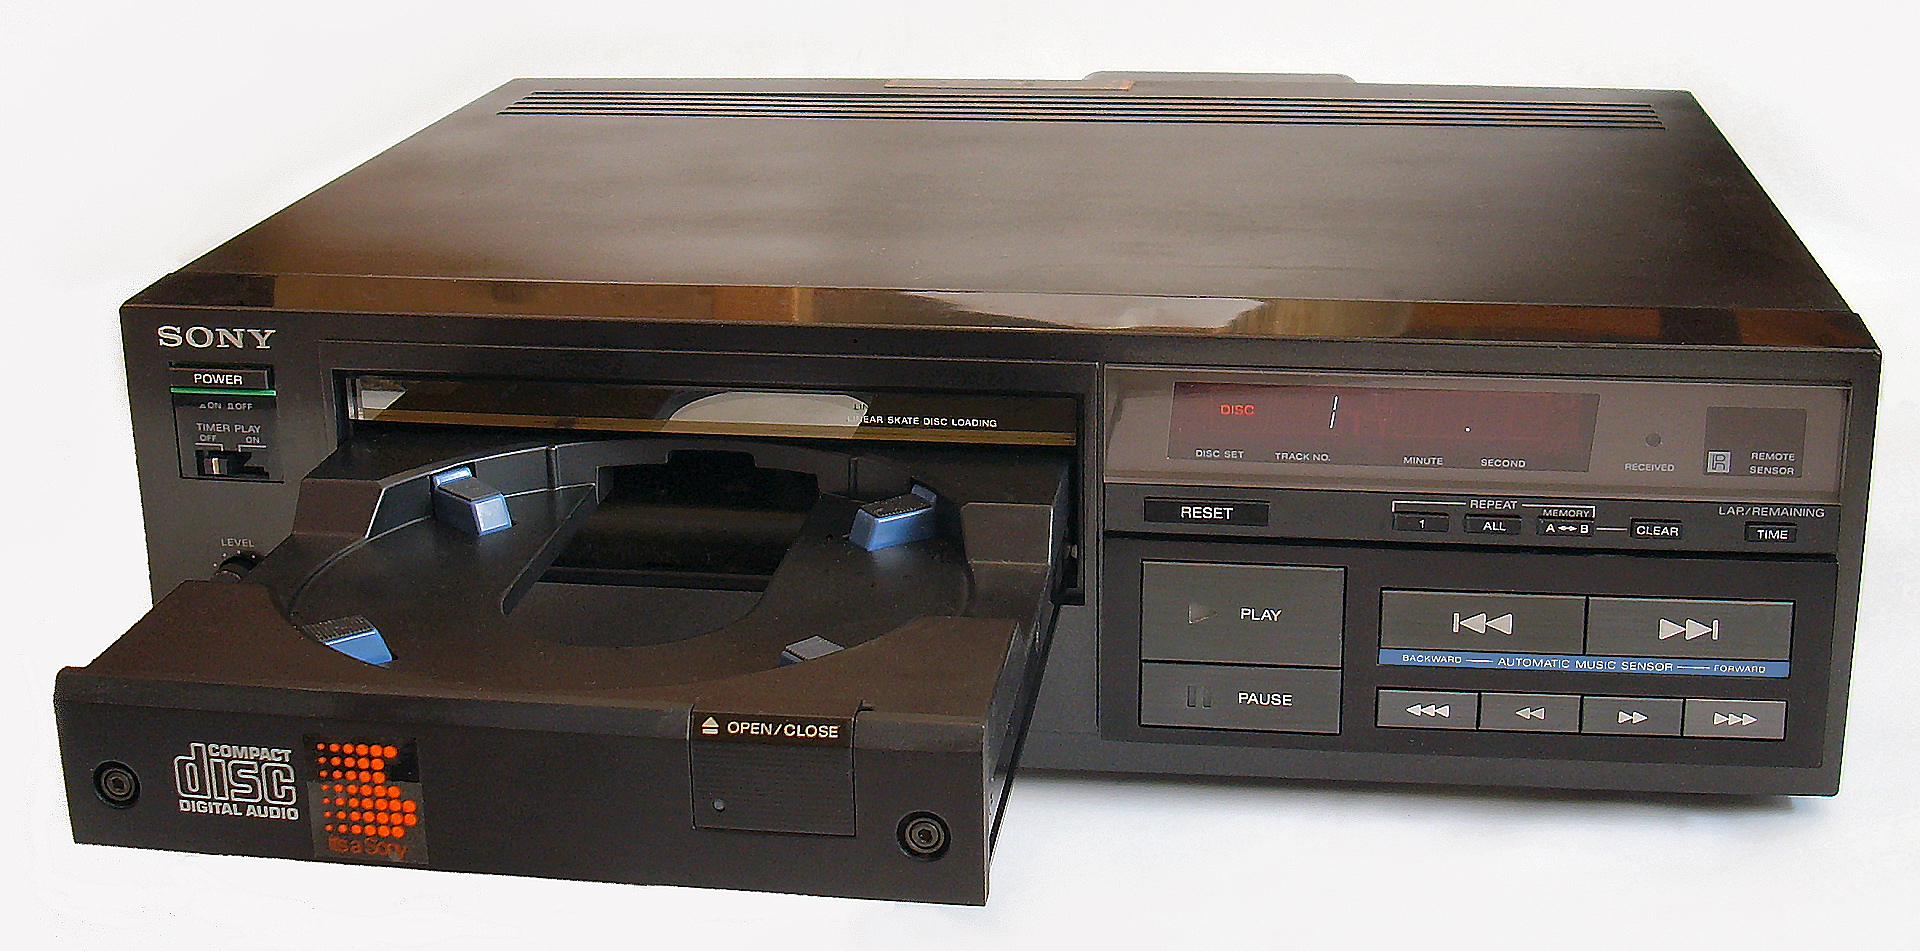
\includegraphics[width=11cm]{res/cd-player.jpg}
	\end{center}
\end{frame}


\section{Inheritance}
\subsection{Inheritance}
\begin{frame}{}
	\begin{center}
		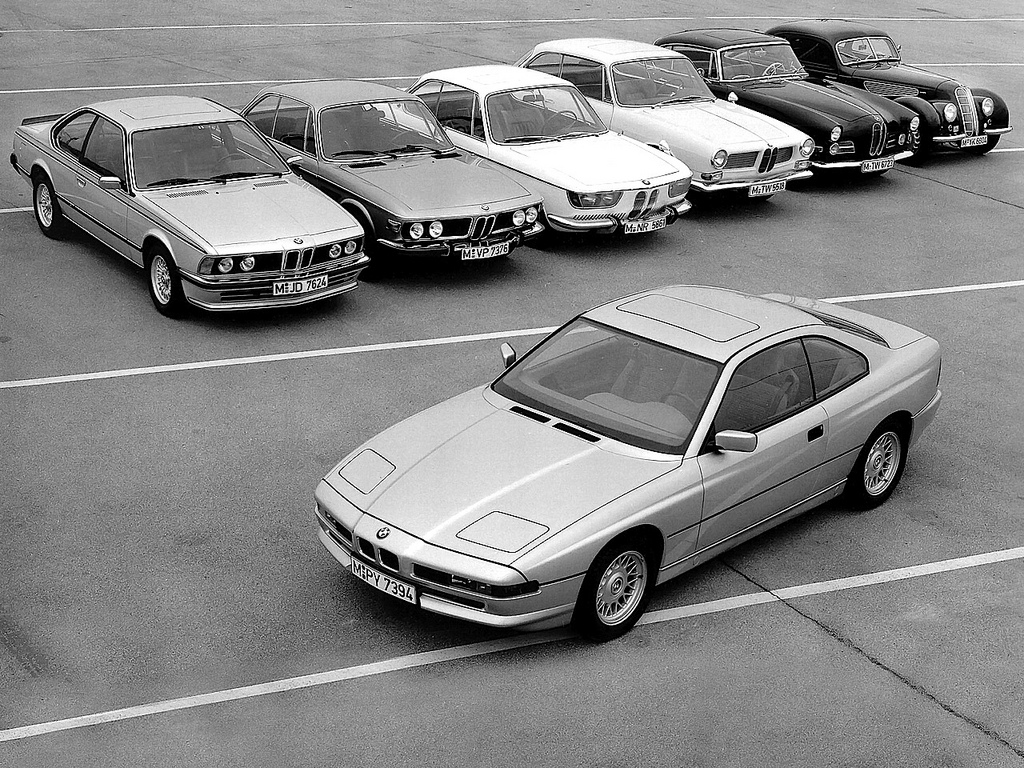
\includegraphics[width=9.5cm]{res/bmw-series.jpg}
	\end{center}
\end{frame}

\begin{frame}{A special Delivery}
	\begin{center}
		
\includegraphics[width=11cm]{res/letterandpackage.jpg}
	\end{center}
\end{frame}




\begin{frame}[fragile]{A special Delivery}
	Our class \emph{Letter} is a kind of \emph{Delivery} denoted by the keyword \textbf{extends}.
	\begin{itemize}
		\item \emph{Letter} is a \textbf{subclass} of the class \emph{Delivery}
		\item \emph{Delivery} is the \textbf{superclass} of the class \emph{Letter}
	\end{itemize}
	\begin{lstlisting}
	public class Letter extends Delivery {
	
	}
	\end{lstlisting}
	\vfill
	As mentioned implicitly above a class can has multiple subclasses. 
	But a class can only inherit directly from one superclass.
\end{frame}

\begin{frame}[fragile]{Example}
	We have the classes: \emph{PostOffice}, \emph{Delivery} and \emph{Letter}.
	They will be used for every example in this section and they will grow over time.
	\begin{lstlisting}
	public class Delivery {
	
	    private String address;
	    private String sender;
	    
	    public void setAddress(String addr) {
			address = addr;
	    }
	    
	    public void setSender(String snd) {
			sender = snd;
	    }
	    
	    public void printAddress() {
	        System.out.println(this.address);
	    }
	}
	\end{lstlisting}
	
	\begin{lstlisting}
	public class Letter extends Delivery {
	
	}
	\end{lstlisting}
\end{frame}

\begin{frame}[fragile]{Inherited Methods}
	The class \emph{Letter} also inherits all methods from the superclass \emph{Delivery}.
	\begin{lstlisting}
	public class PostOffice {
	
	    public static void main(String[] args) {
	    
	        Letter letter = new Letter();
	        
	        letter.setAddress("cafe ascii, Dresden");
	        
	        letter.printAddress();
	        // prints: cafe ascii, Dresden
	    }	
	}
	\end{lstlisting}
\end{frame}

\begin{frame}[fragile]{Override Methods}
	The method printAddress() is now additional definded in \emph{Letter}.
	\begin{lstlisting}[escapechar=!]
	public class Letter extends Delivery {
	
	    @Override
	    public void printAddress() {
	        System.out.println("a letter for " + this.address);    
	    }	
	}
	\end{lstlisting}
	% programer is AE
	\texttt{@Override} is an annotation. 
	It helps the programer to identify overwritten methods.
	It is not neccessary for running the code but improves readability.
	What annotations else can do we discuss in a future lesson.
\end{frame}
\begin{frame}[fragile]{Override Methods}
	Now the method \texttt{printAddress()} defined in \emph{Letter} will be used instead of the method defined
	in the superclass \emph{Delivery}.
	\begin{lstlisting}
	public class PostOffice {
	
	    public static void main(String[] args) {
	    
	        Letter letter = new Letter();
	        
	        letter.setAddress("cafe ascii, Dresden");
	        
	        letter.printAddress();
	        // prints: a letter for cafe ascii, Dresden
	    }	
	}
	\end{lstlisting}
\end{frame}

\subsection{Constructor}
\begin{frame}[fragile]{Super()}
	If we define a \textbf{constructor with arguments} in \emph{Delivery} we have to define a constructor
	with the same list of arguments in every subclass.
	\begin{lstlisting}[basicstyle=\ttfamily\scriptsize]
	public class Delivery {
	
	    private String address;
	    private String sender;
	    
	    public Delivery(String address, String sender) {
	        this.address = address;
	        this.sender = sender;
	    }
	    	    
	    public void printAddress() {
	        System.out.println(address);
	    }
	}
	\end{lstlisting}
\end{frame}

\begin{frame}[fragile]{Super()}
	For the constructor in the subclass \emph{Letter} we can use \texttt{super()} to call the constructor
	from the superclass.
	\begin{lstlisting}[escapechar=!]
	public class Letter extends Delivery {

	    public Letter(String address, String sender) {
	        super(address, sender);
	    }
	
	    @Override
	    public void printAddress() {
	        System.out.println("a letter for " + this.address);    
	    }	
	}
	\end{lstlisting}
\end{frame}

\begin{frame}[fragile]{Super() - Test}
	\begin{lstlisting}
	public class PostOffice {
	    
	    public static void main(String[] args) {	    
	        Letter letter = 
	            new Letter("cafe ascii, Dresden", "");
	        
	        letter.printAddress();
	        // prints: a letter for cafe ascii, Dresden
	    }
	}
	\end{lstlisting}
\end{frame}

\subsection{Implicit Inheritance}
\begin{frame}{Object}
	Every class is a subclass from the class \emph{Object}. 
	Therefore every class inherits methods from \emph{Object}.
	\vfill
	See \scriptsize\url{http://docs.oracle.com/javase/7/docs/api/java/lang/Object.html} \normalsize for
	a full reference of the class \emph{Object}.
\end{frame}

\begin{frame}[fragile]{toString()}
	\emph{Letter} is a subclass of \emph{Object}.
	Therefore \emph{Letter} inherits the method \texttt{toString()} from \emph{Object}.\\
	\texttt{System.out.println(argument)} will call \texttt{argument.toString()} to receive
	a printable String.
	\begin{lstlisting}[escapechar=!]
	public class PostOffice {
	    
	    public static void main(String[] args) {	    
	        Letter letter = 
	            new Letter("cafe ascii, Dresden", "");
	        
	        System.out.println(letter);
	        // prints: Letter@_some_HEX-value_
	        // for example: Letter@4536ad4d
	    }
	}
	\end{lstlisting}
\end{frame}

\begin{frame}[fragile]{Override toString()}
	\begin{lstlisting}[escapechar=!]
	public class Letter extends Delivery {

	    public Letter(String address, String sender) {
	        super(address, sender);
	    }
	
	    @Override
	    public String toString() {
	        return "a letter for " + this.address;
	    }	
	}
	\end{lstlisting}
\end{frame}

\begin{frame}[fragile]{Override toString() - Test}
	\begin{lstlisting}
	public class PostOffice {
	    
	    public static void main(String[] args) {	    
	        Letter letter = 
	            new Letter("cafe ascii, Dresden", "");
	        
	        System.out.println(letter);
	        // a letter for cafe ascii, Dresden
	    }
	}
	\end{lstlisting}
\end{frame}

\begin{frame}{Images stolen at:}
	\tiny
	\begin{itemize}
		\item \textbf{BMW Series} Taken from bmwblog.com
		\item \textbf{CD-Player} Taken from wikimedia.com, Uploaded by Ukexpat
	\end{itemize}
	
\end{frame}



%\section{Visability}
%\subsection{}
%\begin{frame}{}
%\end{frame}

\end{document}